
\documentclass{rapport}
\usepackage{lipsum}
\usepackage{multicol}
\usepackage{listings}
\usepackage{amsmath}   
\usepackage{amssymb}
\usepackage{mathtools}
\usepackage{tabto}
\usepackage{xcolor}
\usepackage{graphicx}
\documentclass{article}
\makeatletter
\renewcommand\paragraph{\@startsection{paragraph}{4}{\z@}%
            {-2.5ex\@plus -1ex \@minus -.25ex}%
            {1.25ex \@plus .25ex}%
            {\normalfont\normalsize\bfseries}}
\makeatother
\setcounter{secnumdepth}{4} % how many sectioning levels to assign numbers to
\setcounter{tocdepth}{4} 
\colorlet{darkGreen}{green!30!black!70!}

\begin{document}

%----------- Informations du rapport ---------

\titre{Simulation d’un émetteur / récepteur ADS-B et décodage
temps réel à l’aide de radio logicielle
} %Titre du fichier .pdf
\UE{ Communications numériques

Codage de canal

Traitement du signal} %Nom de la UE


\sujet{TS229} %Nom du sujet
\enseignant{
            \textsc{FERRE} Guillaume
            \\
            \textsc{TAJAN} Romain
            \\
            \textsc{ELLOUZE} Malek
            
            } %Nom de l'enseignant

\eleves{ 
		\textsc{ABIED} Imad
		\\
		\textsc{AMINE} Wiam
		
		} %Nom des élèves

%----------- Initialisation -------------------
        
\fairemarges %Afficher les marges
\fairepagedegarde %Créer la page de garde


\title{Sections}
\date{27 octobre 2021}

\renewcommand\contentsname{\Huge Sommaire \\ }

\maketitle

\tableofcontents

\newpage
\section{\Large Introduction}

Le projet consiste à mettre en oeuvre une simulation d'un émetteur/récepteur de données ADS-B sous Matlab, gèrer les décodages en temps réel, pour enfin pouvoir afficher des avions survolant l'école.
Il sera alors découpé en trois grandes parties, la couche physique ADS-B, la couche MAC ADS-B et puis l'application des résultats de simulation issus des deux parties précédentes.
\section{\Large Couche physique ADS-B}
\subsection{\Large Prise en main de la chaine de communication ADSB}
\subsubsection{\large Démonstration de l'expression de $s_l$(t)}

\large{D'après l'énoncé:
\begin{equation}
    s_l(t) = \sum\limits_{k \in \mathbb{Z}} p_{b_k}(t - kT_s)
\end{equation}
avec :
$p_{b_k}(t)$ = 
\begin{cases}
p_0(t) &\text{ si } b_k = 0 \\
p_1(t) &\text{ si } b_k = 1
\end{cases}

\vspace{8}
Or, $p_0(t) = 0.5 + p(t)$ et $p_1(t) = 0.5 - p(t)$ (telles qu'elles sont définies dans l'énoncé).

\vspace{8}
Donc \forall $k \in \mathbb{Z}$   $p_{b_k}(t - kT_s)$ = 
\begin{cases}
0.5 + p(t - kT_s) &\text{ si } b_k = 0 \\
0.5 - p(t - kT_s) &\text{ si } b_k = 1
\end{cases}

Enfin, \begin{equation}
    s_l(t) = 0.5 + \sum\limits_{k \in \mathbb{Z}} A_k p(t - kT_s)
    \label{sl_expression}
\end{equation}
avec :
$A_k$ = 
\begin{cases}
1 &\text{ si } b_k = 0 \\
-1 &\text{ si } b_k = 1
\end{cases}
\subsubsection{\large Repésentation des signaux $s_l$(t), $r_l$(t) et $r_m$(t) et déduction du rôle du bloc de décision}
En absence du bruit, pour un signal binaire quelconque, $s_l$(t) est obtenu en joignant les impulsions $p_0$(t) et $p_1$(t) selon que le bit vaut 0 et 1 respectivement, représentées sur une période symbole $T_s$.

\vspace{8}
L'implémentation sur Matlab permet de représenter graphiquement $s_l$(t), $r_l$(t) et $r_m$(t) pour un signal binaire qui vaut [1, 0, 0, 1, 0].

\vspace{8}
D'après FIGURE 1, le signal $s_l$(t) est une succession de portes de largeurs différentes, il sera convolué à des portions de portes, d'où il faut bien s'attendre à ce que le résultat de la convolution soit un signal triangulaire.


\begin{figure}[H]
    \centering
    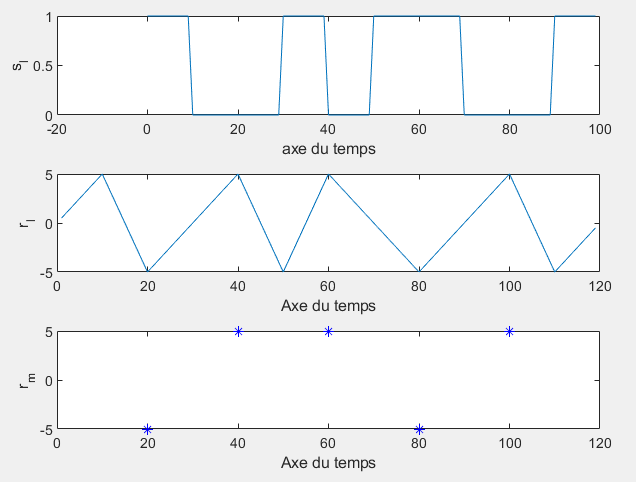
\includegraphics[width=0.7\textwidth]{logos/signaux.PNG}
    \caption{Représentation graphique de $s_l$, $r_l$ et $r_m$ en fonction du temps}
\end{figure}\\

Le bloc de décision permet d'estimer en sortie les symboles et joue également le rôle de l'association "Symbole -> Bits", de sorte qu'à chaque valeur de $r_m$ positive on associe une valeur de bit égale à 0; de même pour une valeur $r_m$ négative, le bit estimé est égal à 1.  

\begin{figure}[H]
    \centering
    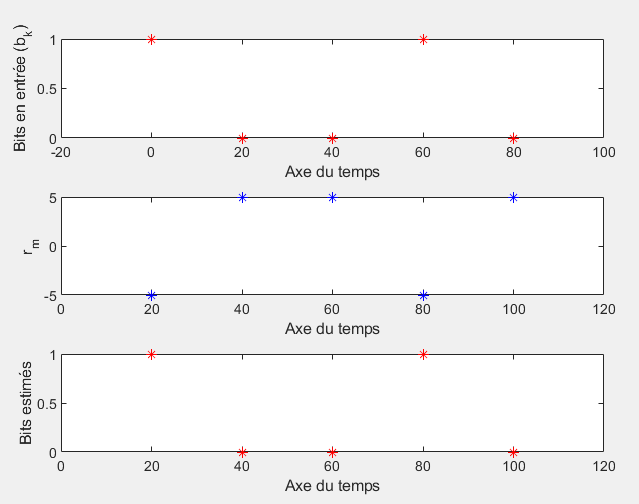
\includegraphics[width=0.7\textwidth]{logos/bits.PNG}
    \caption{Processus de décision et d'estimation des bits selon les valeurs de $r_m$}
\end{figure}\\

\subsubsection{\large Calcul de la probabilité d'erreur binaire $P_b$ pour la modulation PPM en fonction de \frac{$E_b$}{$N_0$}}
\textbf{L’expression de $r_m$ :}

\\
\vspace{8}
\begin{figure}[H]
    \centering
    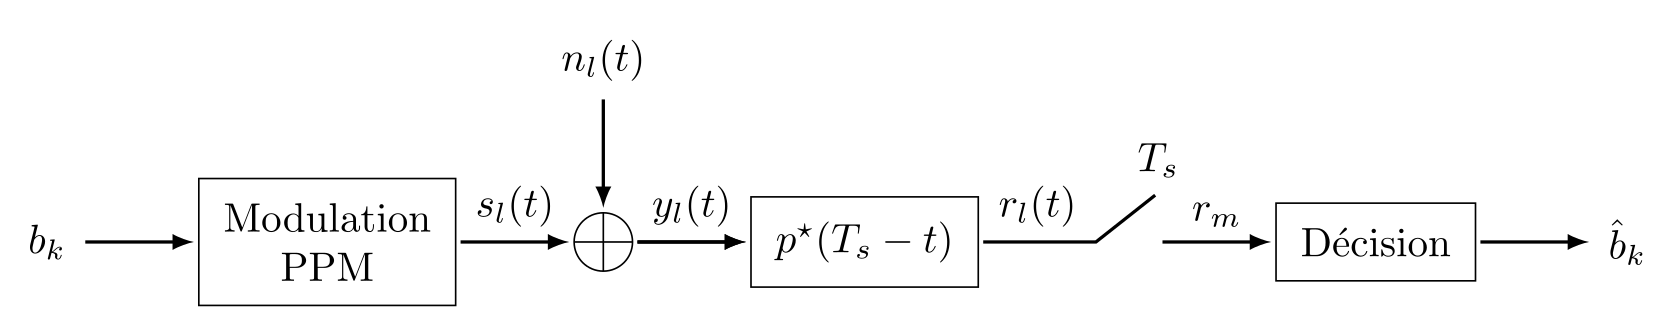
\includegraphics[scale=1]{logos/1_chaine_de_com.png}
    \caption{La chaîne de communication adoptée}
\end{figure}\\
Conformément à la chaîne de communication précédente, on a :

\\
\vspace{8}

$$
\begin{align}
    \mathllap{r_l(t)} &= (0.5 + \sum_{k\in\mathbb{Z}}A_kp(t-kTs))*p^*(Ts-t)\\
    \mathllap{} &= 0.5*p^*(Ts-t) + \sum_{k\in\mathbb{Z}}A_kp(t-kTs)*p^*(Ts-t)\\
    \mathllap{} &= 0.5\int_{-\infty}^{+\infty}p(t)dt + \sum_{k\in\mathbb{Z}}A_kR_p(t-kT_s)
\end{align}
$$
avec $R_p$ la fonction d'autocorrélation de $p$.\\

Donc :
\begin{align}
    r_l(t) = \sum_{k\in\mathbb{Z}} A_kR_p(t-kT_s)
\end{align}

Après l'échantillonnage on a :
$$
\begin{align}
    r_m[n] = r_l(nT_s) = \sum_{k\in\mathbb{Z}} A_kR_p((n-k)T_s)
\end{align}
$$
Comme $p$ respecte le critère de Nyquist, on a $R_p(nT_s) = 0$ pour $n \neq 0$.

\vspace{8}\\
D'où :
\begin{align}
    r_m[n] =A_nR_p(0)
\end{align}
\\
\textbf{L’expression de $P_b$ en fonction de $R_p(0)$ et $\sigma_{n_l'}$ :}
\vspace{8}\\
On note $\sigma_{n_l'}$ l'écart type de $n_l' = n_l * p^*(Ts-t)$. Et $P_b$ la probabilité d'erreur binaire.\\
On a :
$$
\begin{align}
    \mathllap{P_b} &= P(b_n = 1)P(r_m[n] > 0 | b_n = 1) + P(b_n = 0)P(r_m[n] \leq 0 | b_n = 0)\\
    \mathllap{} &= P(r_m[n] > 0 | b_n = 1)\\
    \mathllap{} &= \int_{R_p(0)}^{+\infty} \frac{1}{\sigma_{n_l'}\sqrt{2\pi}}e^{-\frac12(t/\sigma_{n_l'})^2}\\
    \mathllap{} &= \frac12 \frac2{\sqrt\pi}\int_{\frac{R_p(0)}{\sqrt2\sigma_{n_l'}}}^{+\infty}e^{-t²}dt\\
\end{align}
$$

Finalement :
\begin{align}
    \mathllap{P_b} &= \frac12 erfc(\frac{R_p(0)}{\sqrt2 \sigma_{n_l'}})
\end{align}

\\
\textbf{L’expression de $\sigma_{n_l'}$ :}
\vspace{8}\\
On a : $E[n_l'(t)] = \int_{-\infty}^{\infty}E[n_l(x)]p(t-Ts+x)dx = 0$\\
Et :
$$
\begin{align}
    \mathllap{\sigma_{n_l'}^2} &= E[n_l'(t)^2] - E[n_l'(t)]^2\\
    \mathllap{} &=E[\int_{-\infty}^{+\infty}\int_{-\infty}^{+\infty}n_l(x_1)p(t-T_s+x_1)n_l(x_2)p(t-T_s+x_2)dx_1dx_2]\\
    \mathllap{} &=\int_{-\infty}^{+\infty}\int_{-\infty}^{+\infty}p(t-T_s+x_1)p(t-T_s+x_2)E[n_l(x_1)n_l(x_2)]dx_1dx_2\\
    \mathllap{} &=\sigma_{n_l}^2\int_{-\infty}^{+\infty}p(t-T_s+x)p(t-T_s+x)dx\\
\end{align}
$$
Donc :
\begin{align}
    \mathllap{\sigma_{n_l'}^2} &=R_p(0)\sigma_{n_l}^2
\end{align}\\

\\
\textbf{L’expression de $E_b$ en fonction de $R_p(0)$ :}
\vspace{8}\\
Par définition, on a : $E_b = P_{moy}T_s;$ $P_{moy} = \int_{-\infty}^{+\infty}\tau_{s_l}(f)df$\\\\
D'après la formule de Bennett on a : $\tau_{s_l}(f) = \frac1{T_s}|P(f)|^2\sum_{n\in\mathbb{Z}}R_{S_l(n)}e^{-j2\pi fT_s}$\\\\
Avec $R_{S_l}(n) = E[S_l(k)S_l^*(k+n)] = \frac12\delta(0)$\\\\
Donc $P_{moy} = \frac1{2T_s}\int_{-\infty}^{+\infty}|P(f)|^2df = \frac1{2T_s}R_p(0)$\\\\
D'où :
\begin{align}
    \mathllap{E_b} &=\frac12R_p(0)
\end{align}

\\
\textbf{L’expression de $P_b$ en fonction de $\frac{E_b}{N_0}$ :}
\vspace{8}\\

Considérant le fait que $\sigma_{n_l}^2 = \frac{N_0}2$ et d'après les relations précédemment trouvées, on a :
\begin{align}
    \mathllap{P_b(\frac{E_b}{N_0})} &=\frac12erfc(\sqrt{2\frac{E_b}{N_0}})
\end{align}

\subsubsection{\large Représentation de TEB et $P_b$ théorique}
Pour un paquet binaire aléatoire généré uniformément, la courbe de la probabilité d'erreur binaire théorique et celle du taux d'erreur binaire en pratique sont confondues en présence d'un bruit blanc gaussien. Par ailleurs, selon la figure \ref{pb_teb}, on constate qu'à partir d'un rapport $ \frac{E_b}{N_0} $ = 4 dB, la probabilité d'erreur binaire est inférieure ou égale à 3.16x$10^{-5}$.
\begin{figure}[H]
    \centering
    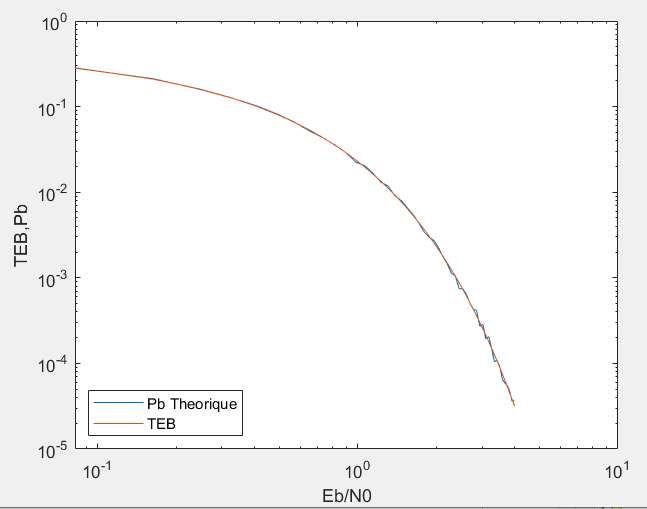
\includegraphics[width=0.8\textwidth]{logos/Pb_TEB.PNG}
    \caption{Représentation de TEB et $P_b$ théorique en fonction du rapport signal sur bruit $ \frac{E_b}{N_0} $}
    \label{pb_teb}
\end{figure}
\subsection{\Large Densité spectrale de puissance}
\subsubsection{\large Calcul du moment d'ordre 1 du signal $s_l(t)$ :}
\\\\
En se basant sur l'équation \eqref{sl_expression} :
$$
\begin{align}
m_{s_l}(t) &= E(s_l(t))\\
           &= E(0.5 +\sum\limits_{k \in \mathbb{Z}} A_k p(t - kT_s))\\
           &= 0.5 + \sum\limits_{k \in \mathbb{Z}} E(A_k) p(t - kT_s)
\end{align}
$$
Or,
$$
\begin{align}
E(A_k) &= 1 . P(A_k = 1) - 1 . P(A_k = -1)\\
       &= 1 . P(b_k = 0) - 1 . P(b_k = 1)\\
       &= \frac{1}{2} - \frac{1}{2} = 0
\end{align}
$$
D'où,
\begin{align}
    m_{s_l}(t) = 0.5
\end{align}

\subsubsection{\large Calcul de la fonction d'autocorrélation du signal $s_l(t)$ :}
$$
\begin{align}
R_{s_l}(t, \tau) &= E(s_l(t)s_l^*(t + \tau))\\
                 &= E((0.5 +\sum\limits_{k \in \mathbb{Z}} A_k p(t - kT_s))(0.5 +\sum\limits_{l \in \mathbb{Z}} A_l^* p^*(t + \tau - lT_s)))\\
                 &= 0.25 + \sum\limits_{k \in \mathbb{Z}}\sum\limits_{l \in \mathbb{Z}} A_k A_l^*p(t - kT_s)p^*(t + \tau - lT_s)\\
                 &= 0.25 + \sum\limits_{k \in \mathbb{Z}}\sum\limits_{l \in \mathbb{Z}} E(A_kA_l^*)p(t - kT_s)p^*(t + \tau - lT_s)\\
                 &= 0.25 + \sum\limits_{k \in \mathbb{Z}}E(\lvert A_k \rvert ^2)p(t - kT_s)p^*(t + \tau - kT_s)\\
                 &= 0.25 + \sum\limits_{k \in \mathbb{Z}}p(t - kT_s)p^*(t + \tau - kT_s)
\end{align}
$$
D'où,
\begin{align}
    R_{s_l}(t, \tau) = 0.25 + \sum\limits_{k \in \mathbb{Z}}p(t - kT_s)p^*(t + \tau - kT_s)
\end{align}


\subsubsection{\large Calcul de l'autocorrélation moyennée du signal $s_l(t)$ en le considérant cyclo-stationnaire de période $T_s$:}
$$
\begin{align}
  \Tilde{R}_{s_l}(\tau) &= \frac{1}{T_s} \int_{0}^{T_s} R_{s_l}(t, \tau)dt\\
                        &= 0.25 + \frac{1}{T_s} \sum\limits_{k \in \mathbb{Z}} \int_{0}^{T_s} p(t - kT_s)p^*(t + \tau - kT_s)dt\\
                        &= 0.25 + \frac{1}{T_s} \sum\limits_{k \in \mathbb{Z}} \int_{-kT_s}^{(1-k)T_s} p(t)p^*(t + \tau)dt\\
                        &=  0.25 + \frac{1}{T_s} \int_{R} p(t)p^*(t + \tau)dt
\end{align}
$$
Ainsi, 
\begin{equation}
    \Tilde{R}_{s_l}(\tau) = 0.25 + \frac{R_p(\tau)}{T_s}
\end{equation}

\subsubsection{\large Déduction de la DSP de $s_l(t)$ :}
\\\\
Soit $c(\tau)$ la partie continue de $\Tilde{R}_{s_l}$ ; $c(\tau) = 0.25$\\
Modélisant $c(\tau)$ par :\\
\[ c(\tau) = \lim_{\theta\to 0}  0.25\pi_{\theta}(\tau)\]
\\
Avec $\pi_{\theta}(\tau)$ la fonction porte de largeur $\theta$. On a :
\[ TF(\pi_{\theta})(f) = \frac{sin(\pi f \theta)}{\pi f} = \theta sinc(\pi f \theta) \underset{\theta \to +\infty}{\rightarrow} \delta(f) \]
\\
Donc :
\[ TF(0.25)(f) = 0.25 \lim_{\theta \to +\infty} TF(\pi_{\theta})(f) \]
\\D'où :
\begin{align}
     TF(0.25)(f) = 0.25\delta(f)
     \label{tf_0_25}
\end{align}

Pratiquement, $c(t)$ est fenêtrée par une fenêtre de largeur nfft. La conséquence de cela dans le domaine spectrale n'est pas négligeable comme la figure \ref{dsp_issue} montre.

\begin{figure}[H]
    \centering
    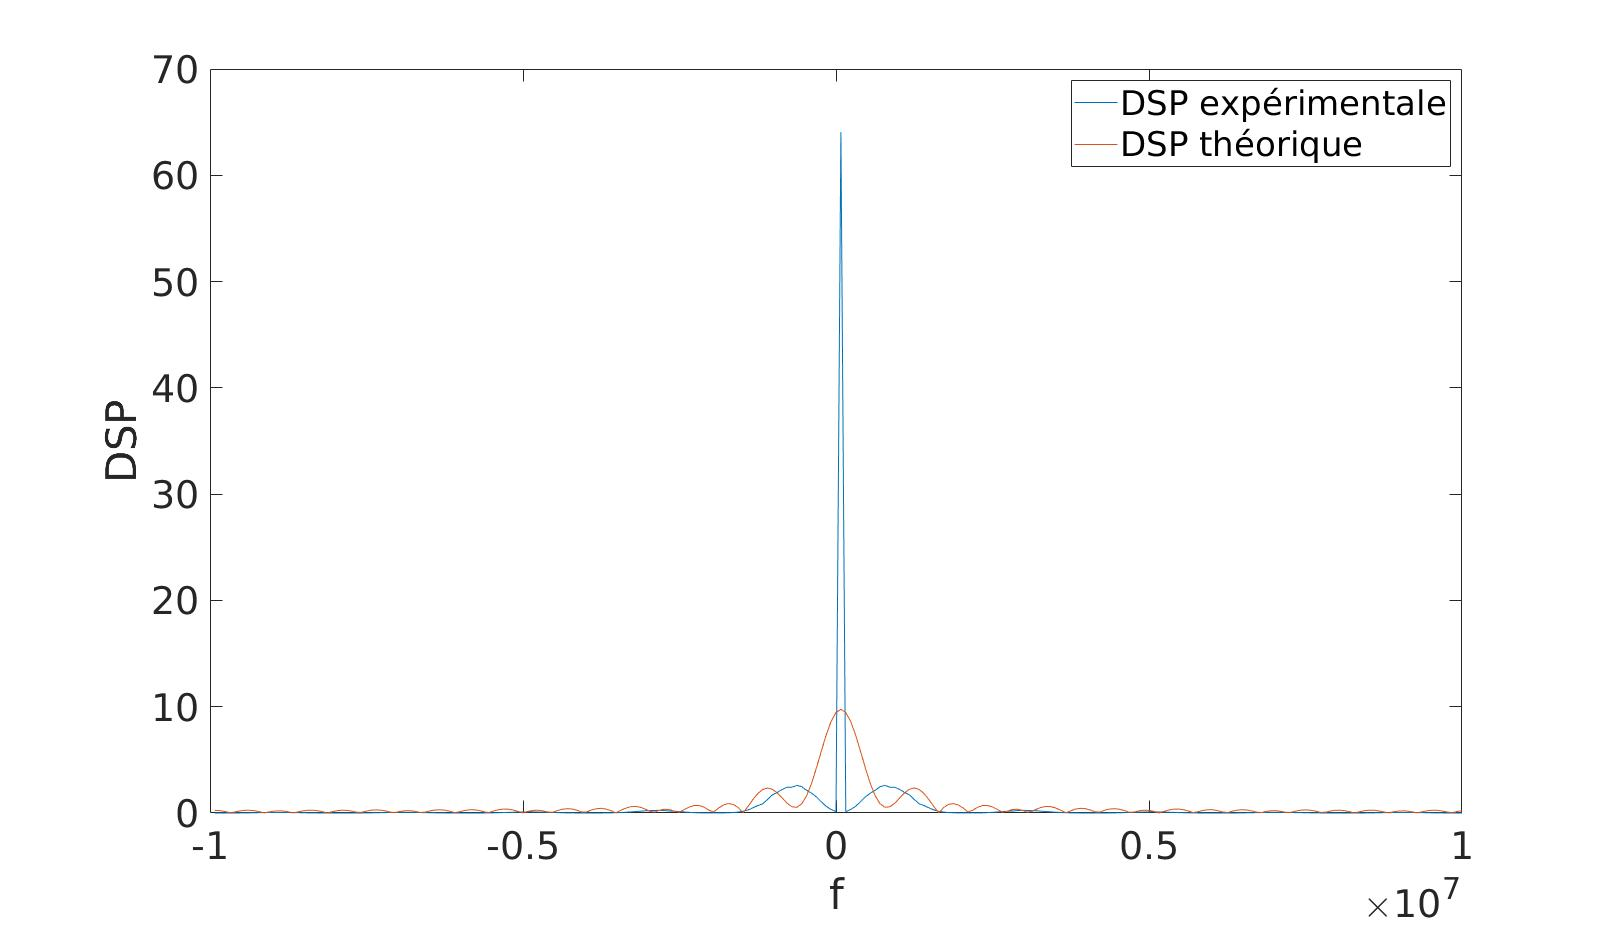
\includegraphics[width=0.7\textwidth]{logos/2_dsp_theo_vs_exper_issue.jpg}
    \caption{Représentation de DSP théorique et DSP expérimentale en fonction de la fréquence}
    \label{dsp_issue}
\end{figure}

Pour palier ce problème, nous proposons d'utiliser la relation \eqref{tf_0_25} avec le remplacement de $\delta$ par $nfft\delta_n$ pour rester fidèle au théorème de Parserval.\\
On définit $\delta_n$ par :
$\delta_n(f)$ = 
\begin{cases}
1 &\text{ si } f = 0 \\
0 &\text{ sinon }
\end{cases}
\\
Le résultat obtenu grâce à cette approche est présenté dans la figure \ref{dsp} :
\begin{figure}[H]
    \centering
    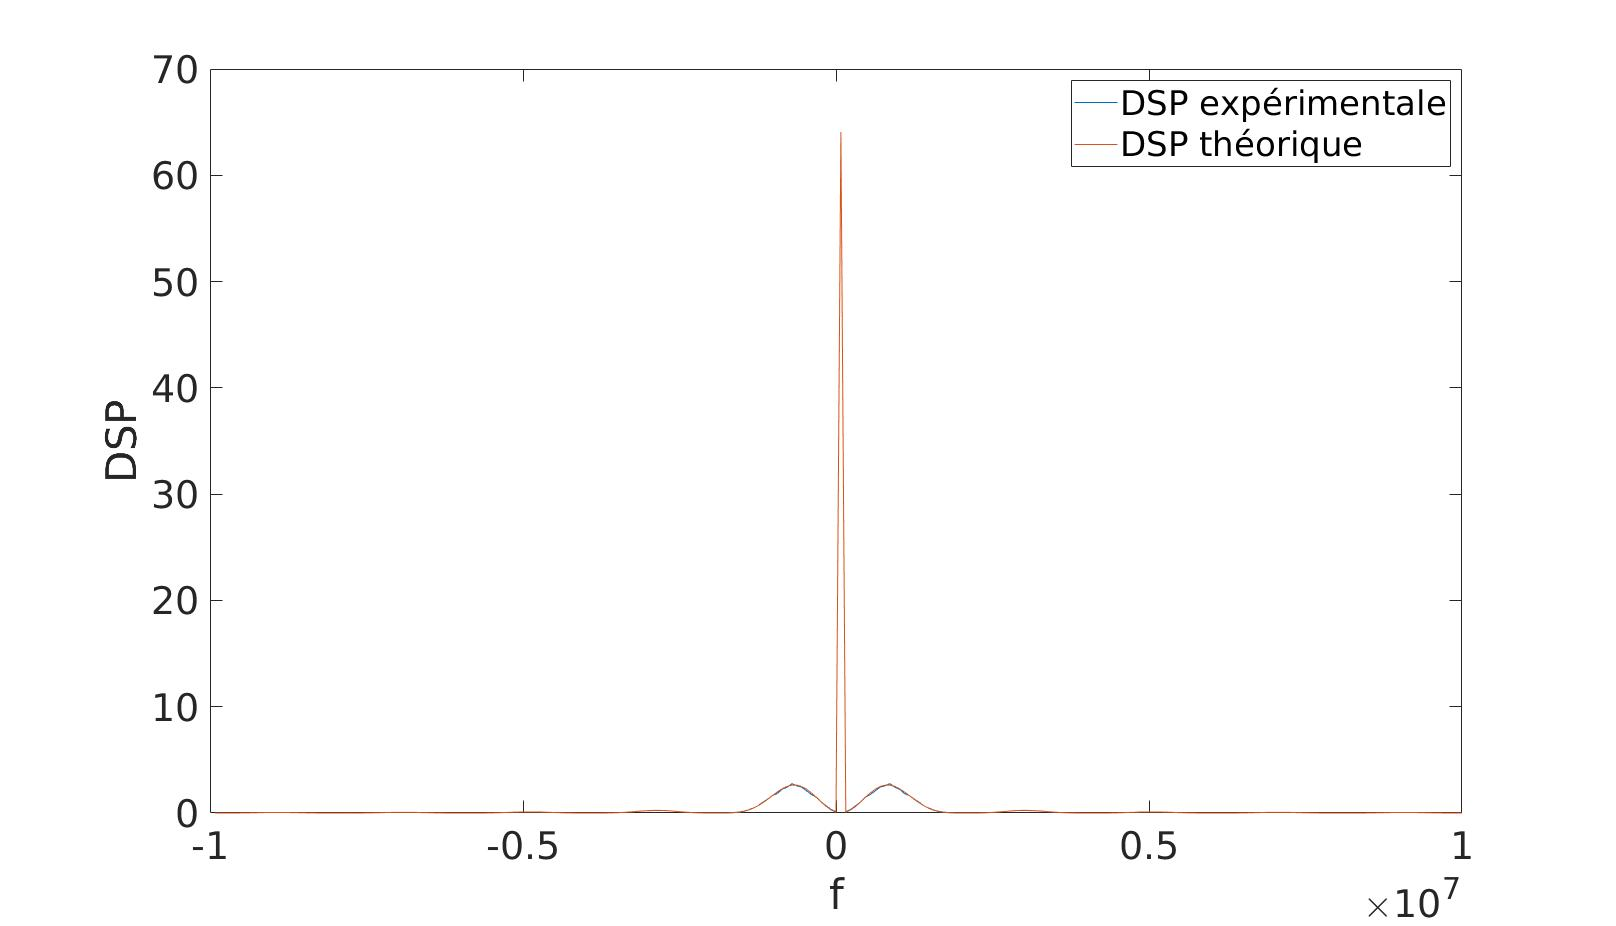
\includegraphics[width=0.8\textwidth]{logos/1_dsp_theo_vs_exper.jpg}
    \caption{Représentation de DSP théorique et DSP expérimentale en fonction de la fréquence}
    \label{dsp}
\end{figure}

\subsection{\Large Algorithmes de codage et de décodage de canal}
Le polynôme fourni à l'énoncé est transformé en une liste de 1 et de 0 selon que le coefficient correspondant à chaque puissance est nul ou pas, cette liste est par la suite passée en paramètre à la fonction \textbf{crc.generator} et puis à \textbf{crc.detector} pour enfin générer les bits de contrôle et les ajouter à la trame.
\vspace{5}

Comme l'énoncé l'annonce, on a pris le soin d'indiquerque le message n'est pas intègre en absence d'erreur et intègre sinon.
\subsection{\Large Synchronisation en temps}
Cette partie consiste dans un premier temps à introduire un décalage temporel aléatoire, à estimer ce décalage en calculant le décalage correspondant au maximum réel positif de la corrélation et puis de faire la synchronisation temporelle.
\vspace{5}

La contrainte majeure était de concilier le nombre d'erreur commises avec le temps d'exécution, ceci dit, on a pu rédiger un programme qui fait le moindre d'erreur avec un temps d'exécution d'à peu près deux minutes en fixant à certaines valeurs le rapport signal sur bruit maximal et sa taille (tout en laissant le seuil à 100 erreurs), pour enfin obtenir la représentation ci-dessous.

\begin{figure}[H]
    \centering
    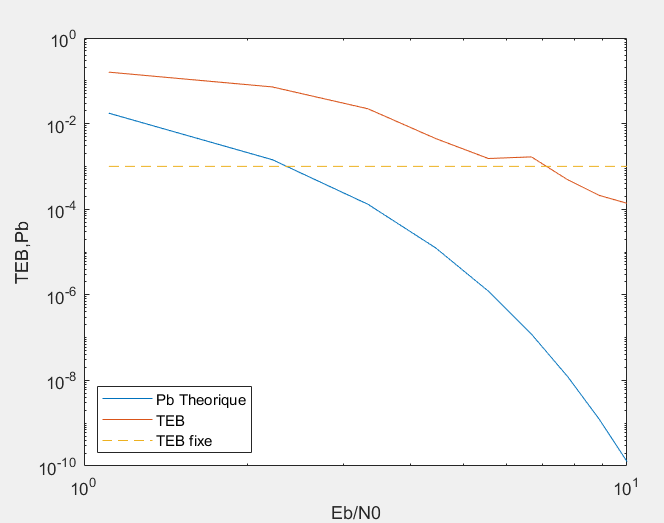
\includegraphics[width=0.7\textwidth]{logos/TEB_Pb.PNG}
    \caption{Représentation du taux d’Erreur Binaire et de la probabilité d'erreur binaire théorique en fonction du rapport signal sur bruit, avec estimation temporelle}
\end{figure}\\

La corrélation en tant que fonction de plusieurs intégrales a été finalement calculée par la méthode des rectangles. En effet, malgré que cette méthodologie pourrait avoir une complexité assez grande, cependant, elle est la plus précise et la plus efficace, la fonction xcorr pour calculer l'inter-corrélation entre le signal $s_p$ et $r_l$ ou même directement la corrélation $\rho$ avec comme troisième paramètre "Normalized" ou "coeff" permet certes d'obtenir un résultat rapidement mais avec un bon nombre d'erreur d'estimation. 
\vspace{5}

L'essentiel était d'obtenir un résultat correct même avec un temps d'attente additionnel.

Les courbes ne se superposent pas suite à la réception de signaux désynchronisés temporellement.

\subsubsection{\large Calcul du décalage de fréquence Doppler d'un avion se déplaçant à vitesse v = 900km/h }

On suppose que le système de diffusion ADS-B se rapproche de la station de réception, les signaux ADS-B sont transmis sur fréquence porteuse $F_p$=1090Mhz, l'effet Doppler fait que l'antenne réceptrice perçoit les signaux à une fréquence différente $F_{ed}=\frac{F_p}{1 + \frac{v}{c}}$ où

c = $3.10^8$.

Etant donné que v < < c, on peut déduire que le décalage fréquentiel $$\Delta F = F_{ed} - F_p \approx \frac{v}{c}.F_p$

Numériquement : $$\Delta F \approx 908.33 Hz$
\subsubsection{\large Calcul du module au carré de $y_l$(t)}
D'après l'énoncé :
\begin{equation}
    y_l(t) = s_l(t-\delta_t)e^{-j2pi\delta_ft} + n_l(t)
\end{equation}
$$
\begin{align}
  \lvert y_l(t) \rvert^2 &= \lvert s_l(t-\delta_t)e^{-j2\pi\delta_ft} + n_l(t) \rvert^2 \\
                        &= \lvert s_l(t-\delta_t)cos(2\pi\delta_ft) + n_l(t) - js_l(t-\delta_t)sin(2\pi\delta_ft)\rvert^2 \\
                        &= (s_l(t-\delta_t)cos(2\pi\delta_ft) + n_l(t))^2 + s_l(t-\delta_t)^2sin^2(2\pi\delta_ft)\\
                        &= s_l(t-\delta_t)^2 + n_l(t)^2 + 2n_l(t)cos(2\pi\delta_ft)s_l(t-\delta_t)
\end{align}
$$
Par ailleurs,
\begin{equation}
    \lvert y_l(t) \rvert^2 =  s_l(t-\delta_t)^2 + z_l(t)
\end{equation}

où $z_l(t) =  n_l(t)^2 + 2n_l(t)cos(2\pi\delta_ft)s_l(t-\delta_t)$

\vspace{6}
La moyenne de $z_l(t)$ n'est pas nulle

$E(z_l(t)) = E(n_l(t)^2) + 2E(n_l(t))cos(2\pi\delta_ft)s_l(t-\delta_t)
                                    = \sigma_n_l$
                                    
\subsubsection{\large Démonstration de l'inégalité $\lvert \rho(\delta_t^{'}) \rvert \leq 1$ $\forall$ $\delta_t^'$ et étude du cas d'égalité}
On sait que $\forall$ $\delta_t^'$

\begin{align}
 \displaystyle\left\lvert \int_{\delta_t^{'}}^{\delta_t^{'} + T_p} r_l(t)s_l^*(t - \delta_t^{'}) dt \displaystyle\right\rvert 
                        \leq \int_{\delta_t^{'}}^{\delta_t^{'} + T_p} \lvert r_l(t) \rvert \lvert s_l^*(t - \delta_t^{'})\rvert dt 
\end{align}

En se basant sur l'inégalité de Cauchy Schwartz :
$$
\begin{align}
< \lvert r_l(t) \rvert,  \lvert s_l(t - \delta_t^{'})\rvert> 
                        &= \int_{\delta_t^{'}}^{\delta_t^{'} + T_p} \lvert r_l(t) \rvert \lvert s_l^*(t - \delta_t^{'})\rvert dt \\
                        &\leq \sqrt{\int_{\delta_t^{'}}^{\delta_t^{'} + T_p} \lvert r_l(t) \rvert^2 dt} \sqrt{ \int_{\delta_t^{'}}^{\delta_t^{'} + T_p}\lvert s_l^*(t - \delta_t^{'})\rvert^2 dt} \\
                        &\leq \sqrt{\int_{\delta_t^{'}}^{\delta_t^{'} + T_p} \lvert r_l(t) \rvert^2 dt} \sqrt{ \int_{0}^{ T_p}\lvert s_l^*(t)\rvert^2 dt}  \\ &$(changement de variable)$
\end{align}
$$
Selon l'équation (15), on peut déduire que $\forall$ $\delta_t^'$ 

$\lvert \rho(\delta_t^{'}) \rvert = \displaystyle\left\lvert \frac{\int_{\delta_t^{'}}^{\delta_t^{'} + T_p} r_l(t)s_l^*(t - \delta_t^{'}) dt }{\sqrt{\int_{\delta_t^{'}}^{\delta_t^{'} + T_p} \lvert r_l(t) \rvert^2 dt} \sqrt{ \int_{0}^{ T_p}\lvert s_l^*(t)\rvert^2 dt}} \displaystyle\right\rvert \leq 1 $



\subsection{\Large Synchronisation en fréquence}
L'effet Doppler introduit également un décalage en fréquence $\delta_f^{'}$. Ainsi pris en compte, la corrélation devient fonction de deux paramètres :

{\Large $\rho(\delta_t^{'}, \delta_f^{'}) =  \frac{\int_{\delta_t^{'}}^{\delta_t^{'} + T_p} e^{j2\pi\delta_f^{'}t} y_l(t)s_l^*(t - \delta_t^{'}) dt }{\sqrt{\int_{\delta_t^{'}}^{\delta_t^{'} + T_p} \lvert y_l(t) \rvert^2 dt} \sqrt{ \int_{0}^{ T_p}\lvert s_l^*(t)\rvert^2 dt}} $}

le signal $y_l(t)e^{j\pi\delta_f^{'}t}$ porte l'information à la fois sur le décalage en fréquence et en temps (à l'encontre du signal $r_l$(t)).
\section{\Large Couche MAC ADS-B}
\subsection{\Large Implémentation de la couche MAC}
\subsubsection{Structure des trames ADS-B}
D'après les données de l'annexe, les valeurs de FTC correspondant à des trames de position de vol varient entre 9 et 18 et entre 20 et 22, tandis que celles correspondant aux messages d'identifications varient entre 1 et 4.
\section{\Large Application}
\subsubsection{Récupération des enregistrements de buffer.mat}
Cette partie consiste à parcourir les 9 colonnes de buffer.mat, d'en extraire à chaque fois un enregistrement de même taille que le préambule ($8Fse$), et puis calculer la corrélation avec le signal $s_p$, celle-ci est par la suite comparée avec un seuil bien fixé, selon qu'elle soit supérieure ou inférieure, on la garde et on passe au décodage de l'enregistrement suivant grâce à la fonction bit2registre. Celle-ci accède aux différentes informations relatives à la trame notamment la latitude, la longitude qui seront stockées dans un tableau.

Cependant, la gestion du seuil ne semble pas être pertinente, du fait qu'elle est restreinte entre 0 et 1, d'où le choix d'afficher les points les plus corrélés avec le préambule (20 points). 

\subsubsection{\Large Traitement de signaux réels}
Les figures suivantes représentent les avions obtenus à partir du fichier buffers.mat ainsi qu'un encadrement du seuil de corrélation calculé à l'issue de chaque 2O points (comme déjà mentionné).
Enfin, il semble que le bon seuil de détection est compris entre 0.73 et 0.82.

\begin{figure}[H]
    \centering
    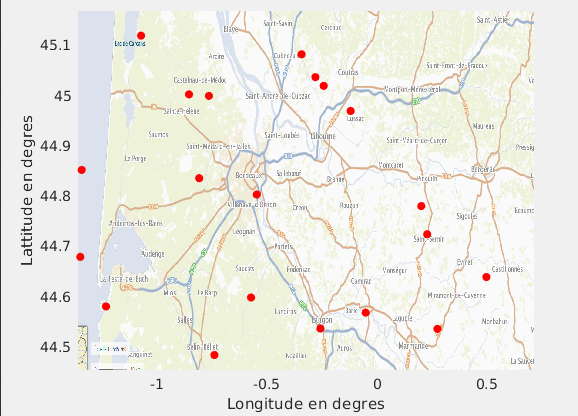
\includegraphics[width=0.66\textwidth]{logos/tache_8_2_map.png}
    \caption{Points obtenus à partir du fichier buffer.mat}
    \label{pb_teb}
\end{figure}

\begin{figure}[H]
    \centering
    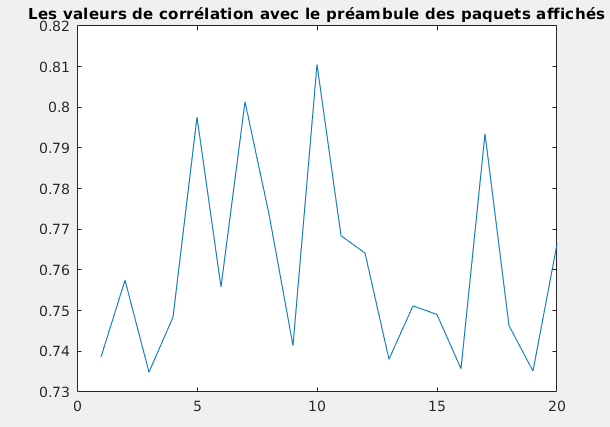
\includegraphics[width=0.66\textwidth]{logos/tache_8_2_corr_val.png}
    \caption{Intervalle des bonnes valeurs du seuil de détection}
    \label{pb_teb}
\end{figure}






\newpage
\section{\Large Conclusion}
Au cours du projet, on a pu concilier théorie et pratique grâce à des notions variées vues en cours de première et deuxième année de télécommunications, ceci nous a été favorable dans la mesure où on a pu approfondir nos connaissances en communications numériques et gagner un socle de connaissance sur les notions de codage, décodage et chaînes de communication.


\section{\Large Références}
- \href{https://gnuradio-fr-18.sciencesconf.org/data/pages/ADSB_TP.pdf}{Application au décodage des signaux ADS-B.}
\vspace{7}

- \href{http://maths-sciences-lp.ac-amiens.fr/IMG/dossier_radar/doppler_dossier.pdf}{Radars et effet Doppler}
\vspace{7}

- \href{https://fr.mathworks.com/help/comm/ref/crc.detector.html}{Manuel CRC.detector}
\vspace{7}

- \href{https://perso.esiee.fr/~bercherj/New/pubs/Bouquin/Synchro.pdf}{Synchronisation}
\vspace{7}

- \href{http://www.aero-hesbaye.be/dossiers/informations/ADS-B.html}{L'ADS-B}
\vspace{7}

- \href{https://docplayer.fr/58073487-Conception-d-un-recepteur-de-donnees-ads-b-pour-la-surveillance-du-reseau.html}{conception d'un récepteur de donnée ADS-B}
\vspace{7}

- Cours Communications numériques première année.
\vspace{7}

- Cours traitement de l'image.
\vspace{40}

\textbf{FIN}

\end {document}